\section{Lezione 22}

Un problema grosso nella produzione del codice � che non siamo in generale preparati ad avere una buona strategia di \textbf{gestione degli errori}:

\begin{itemize}

	\item \textbf{Relativi al flusso di dati}: non posso assumere che l'utente inserisca sempre dati corretti, ma allo stesso tempo non posso accettare \textit{spazzatura}. Sugli input non posso fare assunzioni ottimistiche. Problematiche relative alla disponibilit� di un dato;
	\item \textbf{Relativo al flusso di controllo}: le azioni che avvengono, gestione di eccezioni che io sollevo o che il sistema genera. Le eccezioni sono problemi che rendono il flusso di controllo instabile, e devo avere una strategia di gestione, altrimenti possono essere dannose;
	\item \textbf{Relative al trascorrere del tempo}: ci possono essere degli impegni che il programma si � preso nei confronti dell'utente (es. mi aspetto che il programma risponda in tot secondi). Devo mettere quindi un limite rispetto al quale mi aspetto qualcosa. L'utente si immagina che il sistema garantisca delle funzionalit� in un tempo finito.

\end{itemize}

Mai programmare e progettare immaginando che le cose vadano a buon fine, fare sempre delle assunzioni pessimistiche. Si pu� fare progettazione parallela solo se ho costruito un'architettura progettuale che garantisca il disaccoppiamento. Devo garantire l'integrit� concettuale, desiderabile in ogni architettura di sistema. L'architettura non � \textit{assembleare}, si fanno scelte su buone norme di progettazione che stanno all'architetto (progettista). Il raccordo tra programmazione e progettazione deve essere esplicito, ci deve essere coerenza. \textbf{Enforce intentions}, l'atto di assicurarsi conformit�, ``fai in modo che il codice realizzi precisamente le indicazioni della progettazione''. Ci� che dico nell'architettura deve essere vero nel codice. La programmazione non deve fare scelte libere, ma rispettare la progettazione. Fare \textbf{programmazione difensiva}, essere esplicitamente pronti a trattare errori, si fa in due modi:

\begin{itemize}

	\item \textbf{Incapsulamento degli errori}: in tutti i luoghi del codice dove so che posso non avere successo devo poter gestire l'errore. Programmare esplicitamente il trattamento dei possibili errori, \textbf{errori dei dati in ingresso} ed errori logici;
	\item La strategia di trattamento va prevista nella progettazione.

\end{itemize}

Metodi di trattamento:

\begin{itemize}

	\item Attendere fino all'arrivo di un valore legale;
	\item Assegnare un valore predefinito (\textit{default});
	\item Usare un valore precedente;
	\item Registrare l'errore in un \textit{log}, per avere un registro di manutenzione;
	\item Sollevare eccezioni (se ho un gestore delle eccezioni);
	\item Abbandonare il programma (se proprio non ce la faccio).

\end{itemize}

Fonti di errori logici:

\begin{itemize}

	\item \textbf{Aritmetica in virgola mobile}: la sua approssimazione pu� cumularsi e condurre a errori importanti e a confronti svianti. Essa � intrisecamente imprecisa, sono operazioni spesso fonti di errore;
	\item \textbf{Puntatori e limiti delle strutture}: i puntatori sono in generale molto pericolosi. Nel momento in cui manipolo indirizzi porto cose ovunque (\textit{segmentation fault}). Devo avere una programmazione che mi garantisca che queste cose non accadano. Voglio imporre che ai dati ci si acceda attraverso \textit{metodi di interfaccia};
	\item \textbf{Allocazione dinamica della memoria}: pu� portare a esaurimento della disponibilit� e alla sovrapposizione di aree sensibili (il garbage collector arriva di tanto in tanto...). Chi fa un programma deve sapere quante \textit{new} pu� fare (oppure non le fa);
	\item \textbf{Ricorsione}: pu� portare all'esaurimento della memoria o alla non terminazione. La ricorsione in ogni applicativo ragionevolmente serio � un concetto \textbf{proibito}, consuma lo stack. La combinazione di \textit{new} e ricorsione � ancora peggio;
	\item \textbf{Concorrenza}: se mal progettata pu� condurre a errori.

\end{itemize}

\textbf{Verifica e validazione}

\begin{itemize}

	\item \textbf{Verifica}: ``ho fatto il sistema nel modo giusto'';
	\item \textbf{Validazione}: ``ho fatto il sistema giusto''.

\end{itemize}

La \textit{software verification} ricerca la completezza e la correttezza del software e tratta ci� che lo supporta. Consente di valutare di conseguenza che il software sia validato. La verifica � a supporto della validazione e la validazione � l'ultima cosa che faccio in un progetto. La verifica � un attivit� che svolgo durante \textbf{tutto lo sviluppo} fino all'ultimo istante dove far� validazione, che servir� a dire che ci� che ho fatto � la cosa giusta. La verifica va fatta per impedire che la risposta finale non sia sbagliata. Devo garantire tre cose importanti:

\begin{itemize}

	\item \textbf{Consistenza}: ``sono ci� che vi attendevate fossi'';
	\item \textbf{Correttezza}: ``ci� che ho conseguito � corretto rispetto alle norme'';
	\item \textbf{Completezza}: ``tutto ci� che ho creato � tutto ci� era atteso''.

\end{itemize}

Sono tre caratteristiche di cui devo accertare l'esistenza su tutti i prodotti parziali dello sviluppo. Il verificatore impara le norme e dice che quello che � stato fornito � fatto come richiesto. Non corregge n� rif� il lavoro ma controlla solo che tutto rispetti le tre caratteristiche. La validazione conseguentemente � una conferma \textbf{by examination}, mostra copertura dei requisiti (utente e software).

\begin{center}
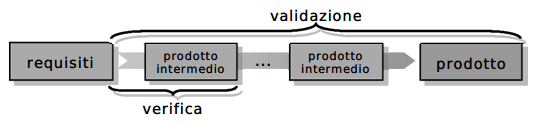
\includegraphics[width=0.75\columnwidth]{img1} % Example image
\end{center}

Le milestone nel progetto didattico sono minimo le revisioni, poi ciascun gruppo pu� fissarne di intermedie.

\begin{center}
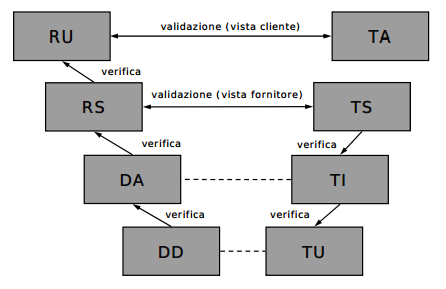
\includegraphics[width=0.75\columnwidth]{img2} % Example image
\end{center}

Per il verificatore ho due forme di \textbf{analisi}:

\begin{itemize}

	\item \textbf{Analisi statica}: non richiede l'esecuzione del programma, studia le caratteristiche del codice sorgente (e a volte anche del codice oggetto);
	\item \textbf{Analisi dinamica}: richiede l'esecuzione del programma, viene effettuata tramite \textbf{test}, usata sia nella verifica che nella validazione.

\end{itemize}

Fissare alcune caratteristiche dell'ambiente dinamico:

\begin{itemize}

	\item \textbf{Ripetibilit�}: � un requisito essenziale. Dobbiamo assumere uno stato inziale prima dell'esecuzione. Il test dev'essere \textbf{deterministico} ed eseguire le cose secondo un ordine noto. Lo stato iniziale � tutto ci� che ha influenza diretta o indiretta sull'esecuzione, e devo sapere qual'�. \textbf{Specifica di un test};
	\item \textbf{Strumenti}:
	\begin{itemize}

		\item \textbf{Driver}: componente attiva fittizia per pilotare una parte;
		\item \textbf{Stub}: componente passiva fittizia per simulare una parte;
		\item \textbf{Logger}: componente non intrusiva di registrazione dei dati di esecuzione per l'analisi dei risultati. Ogni tanto deve lasciare traccia del suo esito.	
	
	\end{itemize}
	\item \textbf{Unit�}: un insieme piccolo di classi che � possibile assegnare a un programmatore. La pi� piccola unit� software che � conveniente verificare singolarmente.

\end{itemize}

\begin{center}
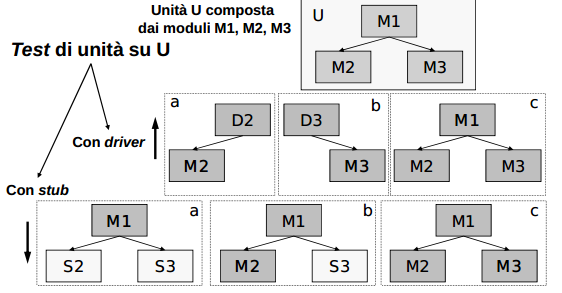
\includegraphics[width=0.75\columnwidth]{img3} % Example image
\end{center}

Una volta verificata ogni singola unit� metto insieme quelle raggruppate e faccio \textbf{test di integrazione}.

\begin{center}
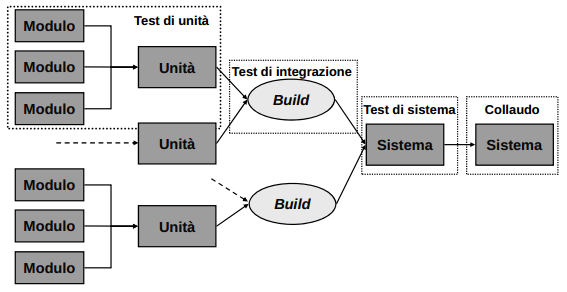
\includegraphics[width=0.75\columnwidth]{img4} % Example image
\end{center}